\subsection{Precisión versus rendimiento}
\label{subsec:resultados2}

\subsubsection{Introducción}

Al analizar nuestra implementación del blur gaussiano en busca de una posible
mejora o variante que pudiera resultar de interés, surgió la idea de cambiar el
tipo de dato en el que se procesaba la imagen. La versión de control utiliza
el tipo float lo cual asegura suficiente precisión al hacer los cálculos, pero a
veces esta precisión no es necesaria y se prefiere un rendimiento mayor en
términos de tiempos de ejecución. Es así como se nos ocurrió estudiar con más
detalle este camino y sus consecuencias.

Para los siguientes experimentos, se utilizó la implementación explicada en la
sección \ref{sec:blur_imp_exp}.

\subsubsection{Hipótesis}

A partir de las ideas mencionadas surgen varios experimentos para intentar
corroborar esta intuición acerca de cómo al sacrificar precisión podemos
posiblemente obtener un filtro de mayor velocidad.

Para empezar, tenemos que al pasar de punto flotante a enteros, dejamos de
tener que realizar conversiones de tipo y realizamos todas operaciones sobre
enteros, que en un principio deberían ser menos costosas que las de punto
flotante. Para esto la primer implementación de prueba que se realizó, difiere
con la de control únicamente en que en lugar de trabajar con floats, lo hace con
enteros de 32 bits, por lo cual procesa la misma cantidad de pixeles en
simultáneo, pero lo hace con instrucciones para enteros.

Por otro lado, si en nuestra versión de control trabajando con floats de 32 bits
operábamos de a un pixel a la vez, con nuestra implementación que utiliza
unsigned short de 16 bits estaríamos procesando dos pixeles en
simultáneo, llevándonos a suponer que esto nos brindaría una disminución en el
tiempo de ejecución a la mitad.

\subsubsection{Metodos utilizados}

Para corroborar nuestra hipotesis generamos un conjunto de imagenes cuadradas
con pixels de colores seleccionados de forma aleatoria, para hacer esto creamos
el archivo llamado random\_images\_generayor.py el cual tiene instrucciones de
uso detalladas en sus comentarios, de todas maneras el funcionamiento de nuestro
blur gaussiano no depende del color de los pixels por lo que se podria haber
utilizado cualquier conjunto de imagenes no necesariamente aleatorias. A partir
de esto creamos imagenes de 5 tamaños distintos, que iban de 25x25 hasta
400x400. Luego repitiendo los experimentos de forma suficiente como para
disminuir la varianza al máximo. Una vez obtenidos estos resultados analizamos
que tanto bajo la calidad de la imagen para esto nos guiamos primero de la mera
observación y complementandolo con el análisis que bmpdiff nos brinda.

Para los experimentos utilizamos tres implementaciones distintas de blur hechas
en assembler estas son explicadas con detalle en la sección de descripción del
codigo.

\subsubsection{Verificación: Experimento 1}


\begin{figure}[H]
\centering
    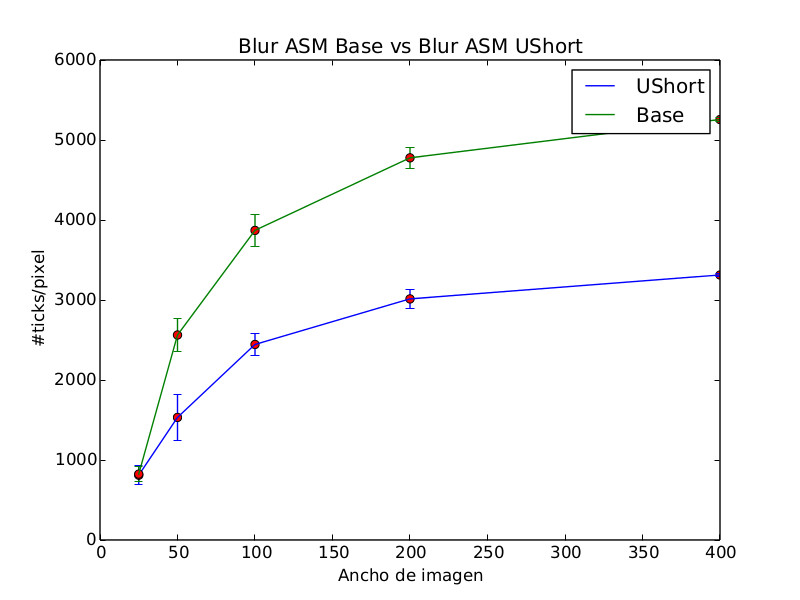
\includegraphics[scale=0.5]{imgs/blur_ushort.jpg}
  \caption{\footnotesize{Grafico donde se observan los tiempo de ejecución de las dos implementaciones estudiadas funcionando con distintos tamaños de imagenes.}}
  \label{fig:tiempo2}
\end{figure}

\begin{figure}[H]
\centering
\begin{minipage}{0.48\textwidth}
  \centering
    
\includegraphics[width=1\textwidth]{imgs/chip_hd_v1.jpg}
  \caption{\footnotesize{Imagen filtrada con blur\_asm\_v1 ($\sigma$ = 3 $r$ = 9), no presenta problemas para mantener el brillo de la imagen.}}
  \label{fig:tiempo1}
\end{minipage}%
\hspace{0.03\textwidth}
\begin{minipage}{0.48\textwidth}
  \centering
    
\includegraphics[width=1\textwidth]{imgs/chip_hd_ushort.jpg}
  \caption{\footnotesize{Imagen filtrada con blur\_asm\_ushort ($\sigma$ = 3 $r$ = 9), la versión que utiliza unsigned short, se nota el oscurecimiento ocasionado probablemente por la perdida de precisión en los cálculos.}}
  \label{fig:tiempo2}
\end{minipage}
\end{figure}


\subsubsection{Verificación: Experimento 2}

Si bien el resultado anterior fue muy prometedor, ya que este mostraba
resultados bastante concluyentes sobre como el tiempo de ejecución habia casi
disminuido a la mitad, de todas maneras notamos que la utilización de unsigned
int en la nueva implementación habia tenido ciertos cambios ajenos al tamaño de
la estructura del dato que podian llegar a contribuir en la velocidad de
computo. La principal sospecha surgió de las instrucciones de conversión de
punto flotante a int (y de int a punto flotante), estas aparecen en
blur\_asm\_v1 pero dejan de ser necesarias en blur\_asm\_ushort.

Para verificar que la influencia de estas instrucciones no era tan grande
implementamos blur\_asm\_uint, esta variante de blur, utiliza unsigned int por
lo que siempre nos mantenemos en representaciones de punto fijo evitando
conversiones. La gran diferencia con la implementación que utiliza shorts es que
el tamaño requerido para hacer los cálculos no va a ser distinto del necesario
en la implementacion base, blur\_asm\_v1.

Los resultados fueron sorpresivos, la influencia de las instrucciones de
conversion parecio casi nula en la velocidad de computa de los programas. Esto
se puede observar en los siguientes gráficos.

\begin{figure}[H]
\centering
    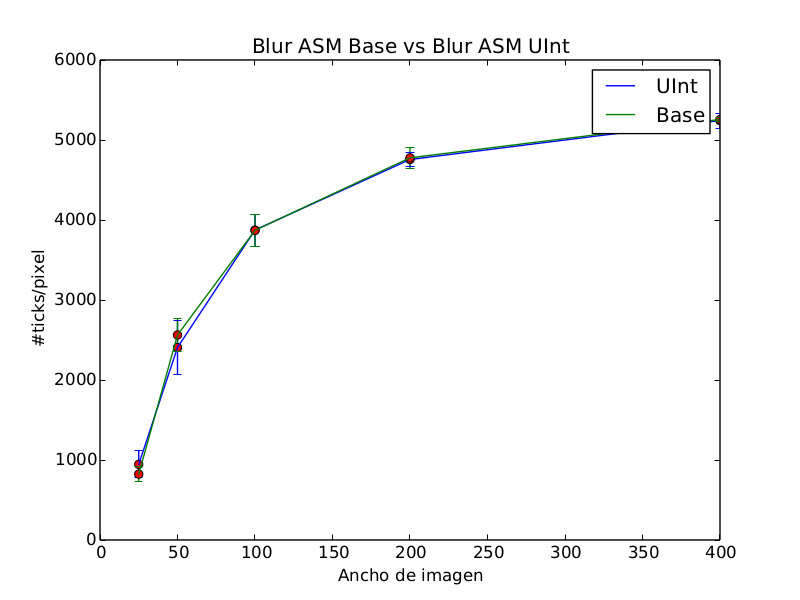
\includegraphics[scale=0.5]{imgs/blur_uint.jpg}
  \caption{\footnotesize{Grafico donde se observan los tiempos de ejecución de las dos implementaciones estudiadas funcionando con distintos tamaños de imagenes.}}
  \label{fig:tiempo1}
\end{figure}

Otro detalle relevante es que observamos como en este caso no se perdia brillo
como pasaba con la implementación de blur UInt, se nota como la mayor cantidad
de bits permiten una precisión suficiente para no redondear tanto los numeros
para abajo y evitando acercarnos a valores cercanos a 0 en la paleta de colores.

\begin{figure}[H]
\centering
    
\includegraphics[scale=0.5]{imgs/chip_hd_uint.jpg}
  \caption{\footnotesize{Imagen filtrada con el blur\_asm\_uint, valores utilizados $\sigma$ = 3 $r$ = 9}}
  \label{fig:tiempo1}
\end{figure}
